\subsection{Connected Component}
For cit-Patents dataset, we found that there are 3627 components in the graph, and the size of the biggest component is 3764117. \\
\\
For soc-Epinions1 dataset, we found that there are 2 components in the graph, and the sizes of components are 75877 and 2. \\
\subsection{Eigenvalue}
cit-patent:\\
\begin{tabular}{ l r }
1 & 53.64209492\\
2 & 10.32982762\\
3 & -5.606214201\\
\end{tabular}
\\
soc-Epinions1:\\
\begin{tabular}{ l r }
1& 241.4042149\\
2 & 17.96681342\\
3 & -14.38048991\\
\end{tabular}
\subsection{K core}
For cit-Patents dataset, we found that there are three 5-cores components in the graph, and the sizes of components are 1847127, 9 and 8. \\
\\
For soc-Epinions1 dataset, we found that there are only one 5-cores components in the graph, and the sizes of components is 16226. \\
\subsection{Degree Distrubutions}

\begin{figure}
\subfloat[In-Degree Distribution\label{fig:cit_indegree}]
  {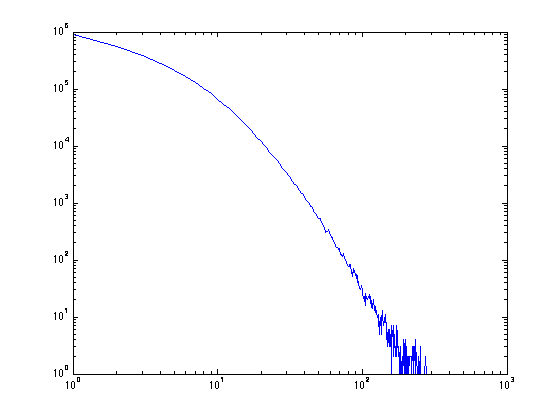
\includegraphics[width=.3\linewidth]{FIG/cit_result/indegreedist.png}}\hfill
\subfloat[Out-Degree Distribution\label{fig:cit_outdegree}]
  {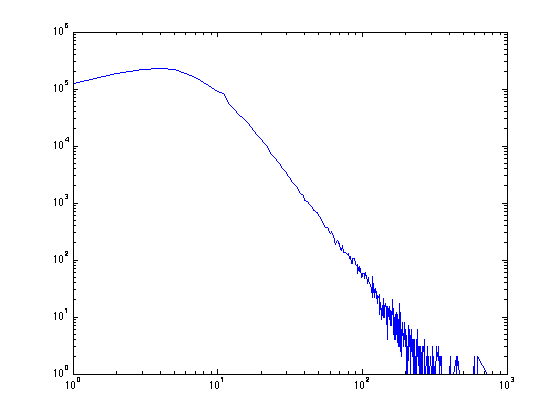
\includegraphics[width=.3\linewidth]{FIG/cit_result/outdegreedist.png}}\hfill
\subfloat[Degree Distribution\label{fig:cit_degree}]
  {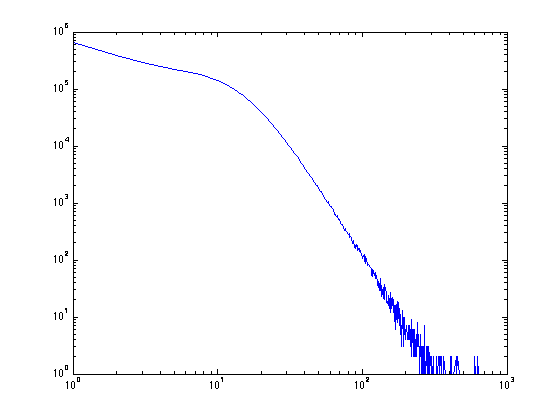
\includegraphics[width=.3\linewidth]{FIG/cit_result/degreedist.png}}
\caption{Degree Distributions of cit-Patents Network\label{fig:cit_degree_dist}}
\subfloat[In-Degree Distribution\label{fig:soc_indegree}]
  {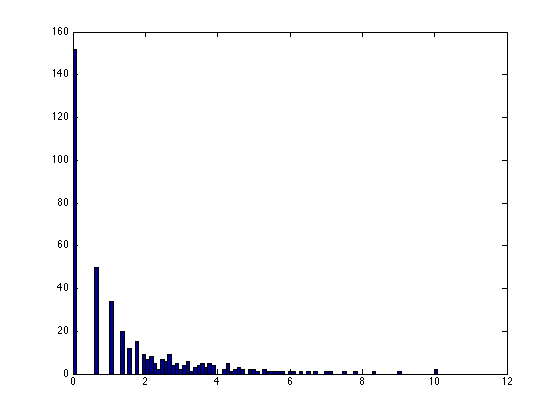
\includegraphics[width=.3\linewidth]{FIG/soc_result/indegreedist.png}}\hfill
\subfloat[Out-Degree Distribution\label{fig:soc_outdegree}]
  {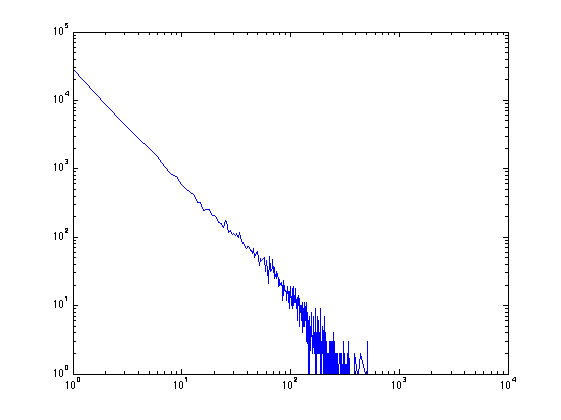
\includegraphics[width=.3\linewidth]{FIG/soc_result/outdegreedist.png}}\hfill
\subfloat[Degree Distribution\label{fig:soc_degree}]
  {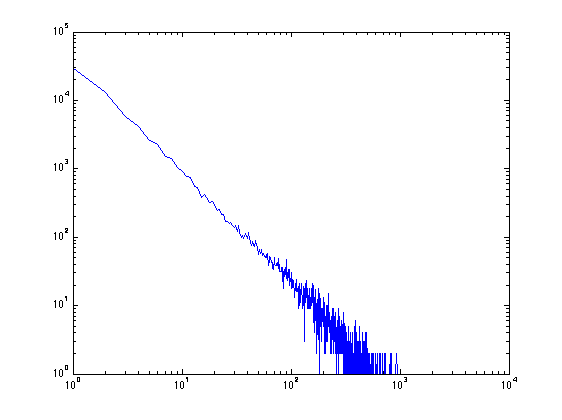
\includegraphics[width=.3\linewidth]{FIG/soc_result/degreedist.png}}
\caption{Degree Distributions of soc-Epinions Network\label{fig:sdegree_dist}}
\end{figure}

According to Figure ~\ref{fig:cit_degree_dist} and Figure ~\ref{fig:sdegree_dist}, we found that the distributions of two networks follow power law. 

\subsection{PageRank and Eigenvector}

\begin{figure}[htbf]
\begin{center}
\begin{tabular}{cc}
     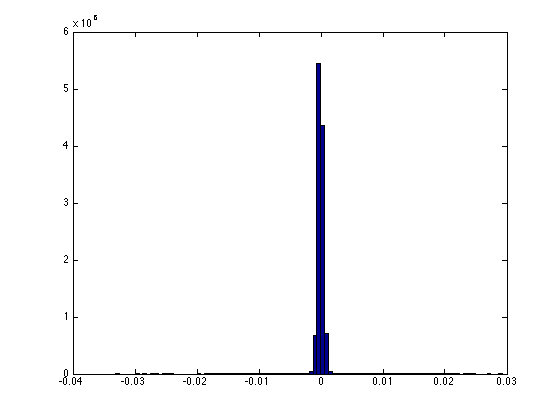
\includegraphics[width=0.5\textwidth]{FIG/cit_result/eigvec.png} &
     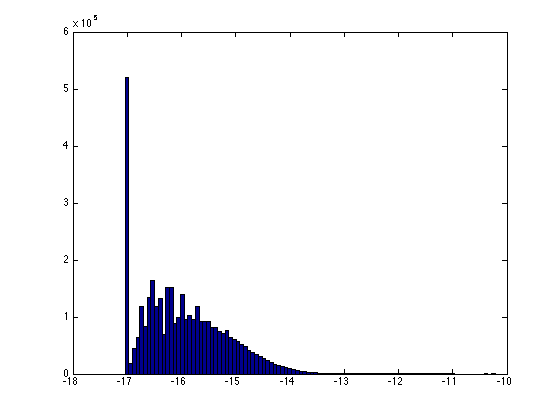
\includegraphics[width=0.5\textwidth]{FIG/cit_result/pagerank.png} \\
    (a) & (b) 
\end{tabular}
\caption{ eigvec (a) and pagerank (b) of cit-Patents}
\label{fig:cit_eigen}
\begin{tabular}{cc}
     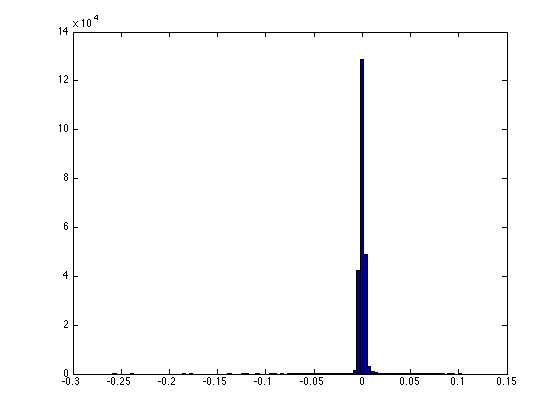
\includegraphics[width=0.5\textwidth]{FIG/soc_result/eigvec.png} &
     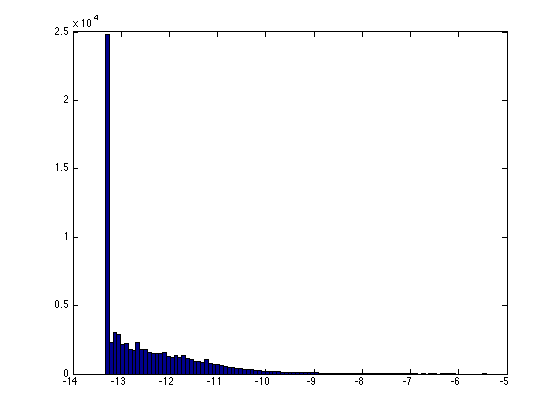
\includegraphics[width=0.5\textwidth]{FIG/soc_result/pagerank.png} \\
    (a) & (b) 
\end{tabular}
\caption{ eigvec (a) and pagerank (b) of soc-Epinions1}
\label{fig:soc_eigen}
\end{center}
\end{figure}

See Figure ~\ref{fig:cit_eigen}  and Figure ~\ref{fig:soc_eigen}. The values of PageRank and Eigenvector are highly skewed.

\subsection{Radius}

\begin{figure}[htbf]
\begin{center}
\begin{tabular}{cc}
     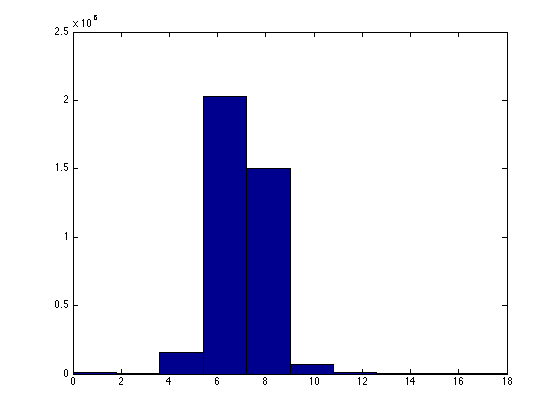
\includegraphics[width=0.5\textwidth]{FIG/cit_result/radius.png} \\
\end{tabular}
\caption{radius of cit-Patents}
\label{fig:cit_radius}
\begin{tabular}{cc}
     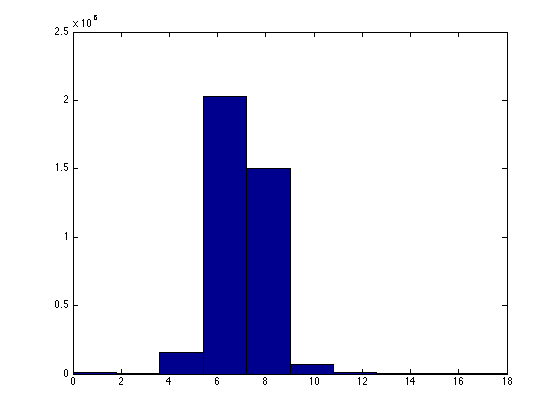
\includegraphics[width=0.5\textwidth]{FIG/cit_result/radius.png} \\
\end{tabular}
\caption{radius of soc-Epinions1}
\label{fig:soc_radius}
\end{center}
\end{figure}

See Figure ~\ref{fig:cit_radius} and Figure ~\ref{fig:soc_radius}. The radius of most of nodes in two networks is 6, which shows that small-word phenomenon exists in two networks. 
